\begin{figure}[h]
    \centering
    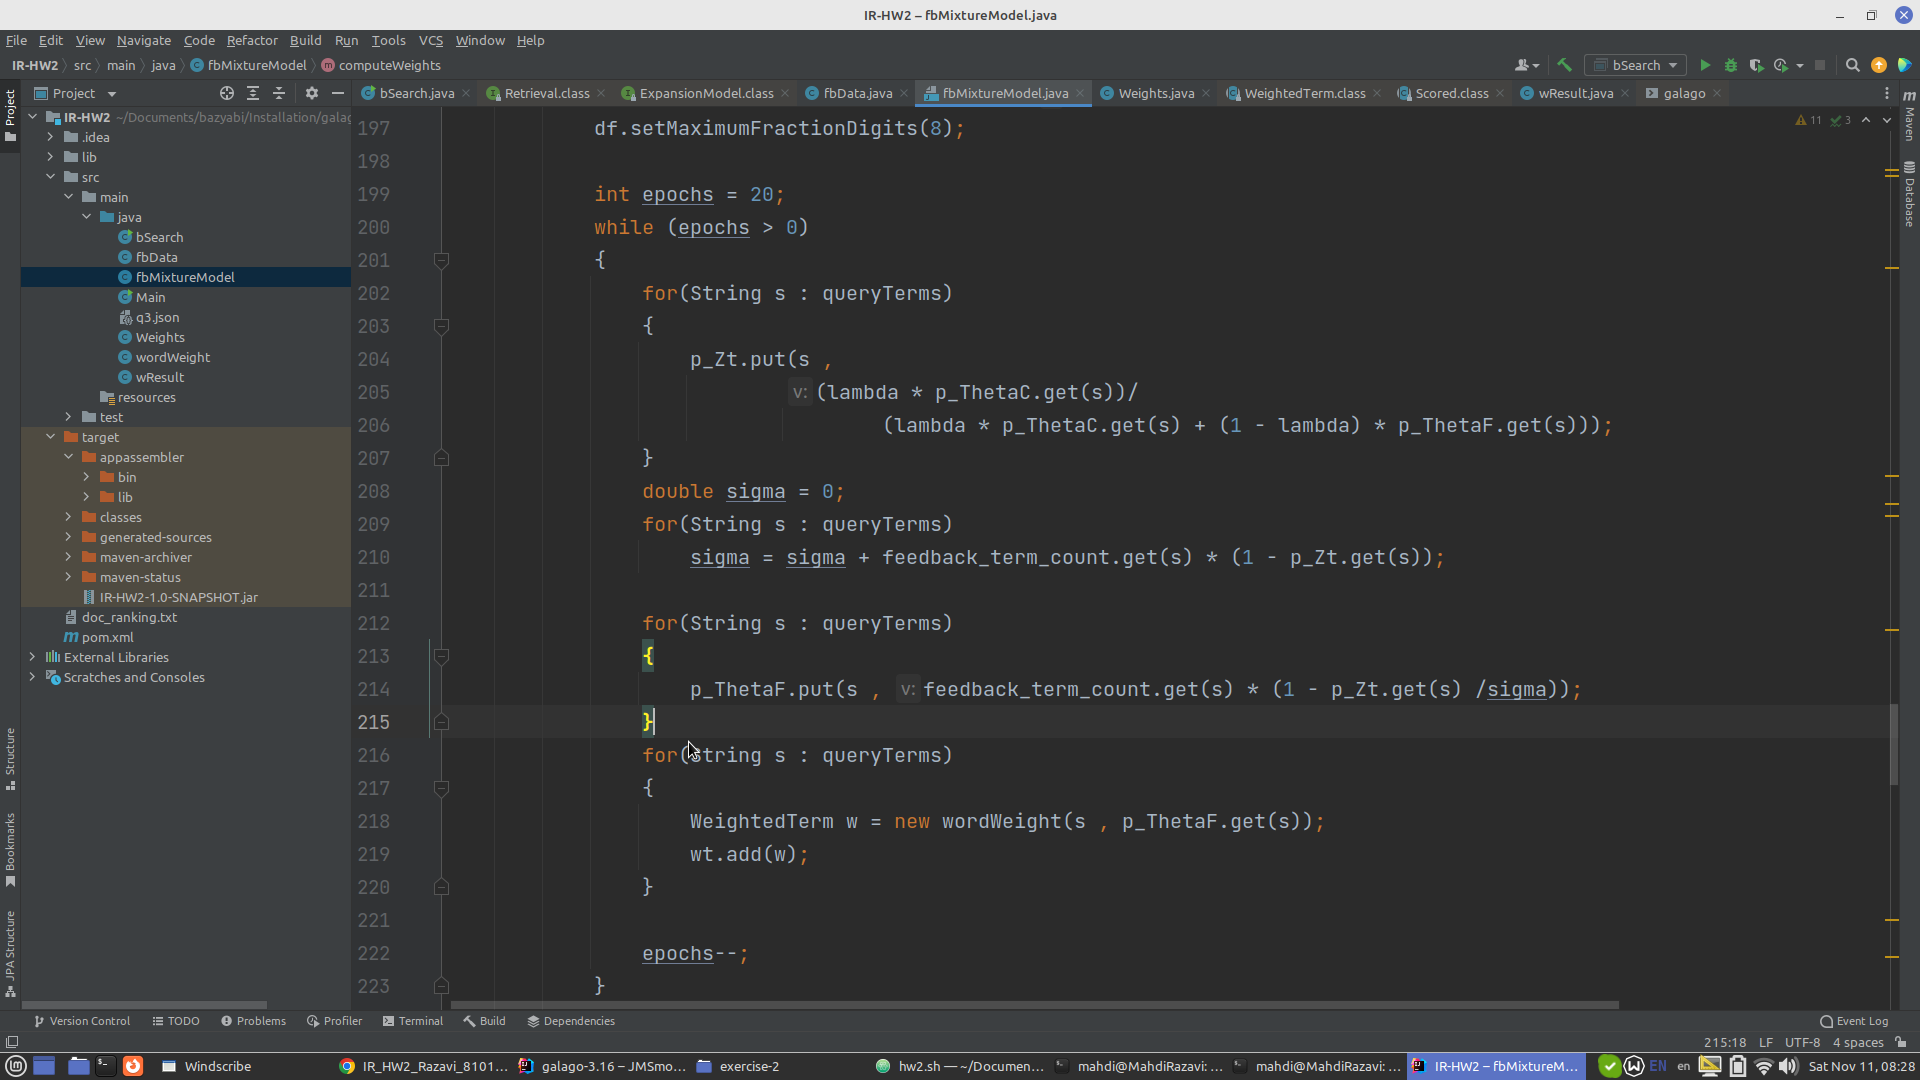
\includegraphics[width=0.8\textwidth]{IR2/images/exercise2-code.png}
    \caption{پیاده‌سازی الگوریتم ترکیبی}
    \label{fig:enter-label}
\end{figure}



\begin{boxC}
    ما الگوریتم ذکرشده در اسلاید درس مبنی بر 
    \lr{EM Computation}
    را پیاده‌سازی کرده‌ایم.

    از ساختمان داده 
    \lr{HashMap}
    برای ذخیره احتمال مورد انتظار و بیشینه احتمال به ازای هر کویری ترم میپردازیم.

    همانطور که در تصویر ارزیابی مشخص است ، نتایج این الگوریتم به طرز معناداری بهتر از روش های هموارسازی های تمرین اول است.

    با اختلاف بیشتر از 
    \lr{0.008} 
    این الگوریتم با حدود 20 بار تکرار به این صورت عمل خواهد کرد.

    به نظر می رسد هر بار تکرار به بیشینه کردن احتمالات تعلق و یا عدم تعلق کلمات مرتبط و نامرتبط کمک خواهد کرد.
\end{boxC}

\begin{figure}[h]
    \centering
    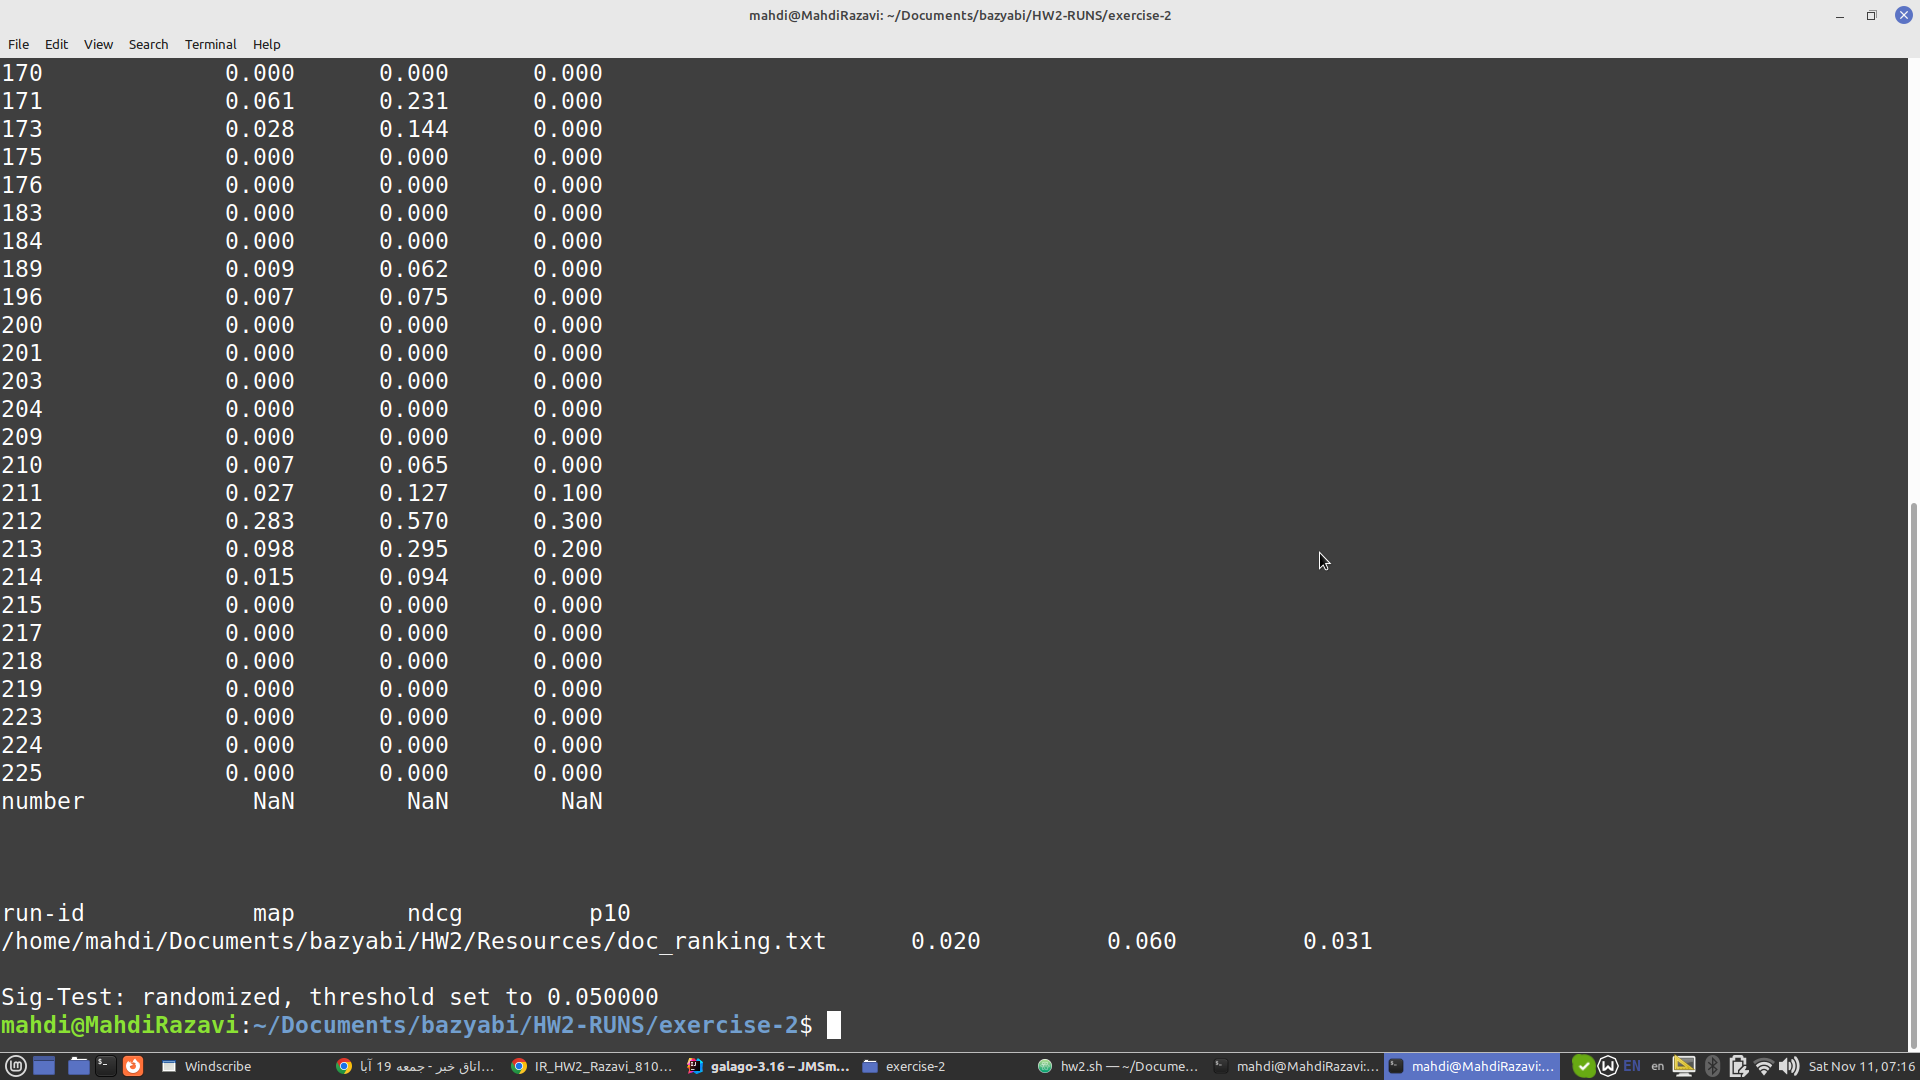
\includegraphics[width=0.8\textwidth]{IR2/images/exercise-2.png}
    \caption{ارزیابی کد بالا}
    \label{fig:enter-label}
\end{figure}

\newpage